\documentclass{VUMIFPSkursinis}
\usepackage{algorithmicx}
\usepackage{algorithm}
\usepackage{algpseudocode}
\usepackage{amsfonts}
\usepackage{amsmath}
\usepackage{bm}
\usepackage{caption}
\usepackage{color}
\usepackage{float}
\usepackage{graphicx}
\usepackage{listings}
\usepackage{subfig}
\usepackage{wrapfig}

\usepackage{enumitem}
%PAKEISTA, tarpai tarp sąrašo elementų
\setitemize{noitemsep,topsep=0pt,parsep=0pt,partopsep=0pt}
\setenumerate{noitemsep,topsep=0pt,parsep=0pt,partopsep=0pt}

% Titulinio aprašas
\university{Vilniaus universitetas}
\faculty{Matematikos ir informatikos fakultetas}
\department{Programų sistemų katedra}
\papertype{Programų sistemų inžinerijos I laboratorinis darbas Nr. 1}
\title{Kavinės staliuko rezervavimo aplikacija}
\titleineng{Cafe table rezervation app}
\status{3 kurso 5 grupės studentai}
\author{Paulius Grigaliūnas}
\secondauthor{Karolis Staskevičius}
\thirdauthor{Modestas Dulevičius}
\fourthauthor{Albert Jurkoit}
\fifthauthor{Šarūnas Kazimieras Buteikis}
     

% \secondauthor{Vardonis Pavardonis}   % Pridėti antrą autorių
\supervisor{dr. Vytautas Valaitis}
\date{Vilnius – \the\year}

% Nustatymai
% \setmainfont{Palemonas}   % Pakeisti teksto šriftą į Palemonas (turi būti įdiegtas sistemoje)
\bibliography{bibliografija}

\begin{document}
	
% PAKEISTA	
\maketitle
\cleardoublepage\pagenumbering{arabic}
\setcounter{page}{2}


%ANOTACIJA

\sectionnonum{ANOTACIJA}
{\bfseries Darbo tikslas:} sukurti išmanų, patogų kavinių staliukų rezervavimo programėlės modelį, kuris funkcionuotų Windows ir Android sistemose. Taip pat siekiama, kad galutinė programėlė užtikritnų sklandų, spartų komunikabilumą tarp klientų ir kavinės darbuotojų, suteikiant galimybę kavinių savininkams pateikti išsamų kavinės planą, o klientams išsirinkti norimą staliuką kavinėje patiems. 
\newline
\newline
\newline

%DARBO ATLIKO

{\bfseries Darbą atliko:}
\newline
\newline
\newline
Paulius Grigaliūnas
\newline
paulius.grigaliunas.pg@gmail.com
\newline
\newline
\newline
Karolis Staskevičius
\newline
karolio paštas
\newline
\newline
\newline
Modestas Dulevičius
\newline
modes paštas
\newline
\newline
\newline
Albert Jurkoit
\newline
alberto paštas
\newline
\newline
\newline
Šarūnas Kazimieras Buteikis
\newline
sarunas.kazimieras.buteikis@gmail.com

%TURINYS

\tableofcontents

%ĮVADAS

\sectionnonum{Įvadas}
\noindent
{\bfseries Programų sistemos pavadinimas}
\newline
tekstas
\newline
\newline
{\bfseries Dalykinė sritis}
\newline
tekstas
\newline
\newline
{\bfseries Probleminė sritis}
\newline
tekstas
\newline
\newline
{\bfseries Naudotojai}
\newline
tekstas
\newline
\newline
{\bfseries Darbo pagrindas}
\newline
tekstas
\newline
\newline

\section{Programų sistemos architektūra}
%LOGINIS PJUVIS
\subsection{Loginis pjūvis}
%KLASIU DIAGRAMA
\subsubsection{Klasių diagrama}

Žemiau pateikta


\begin{figure}[H]
    \centering
    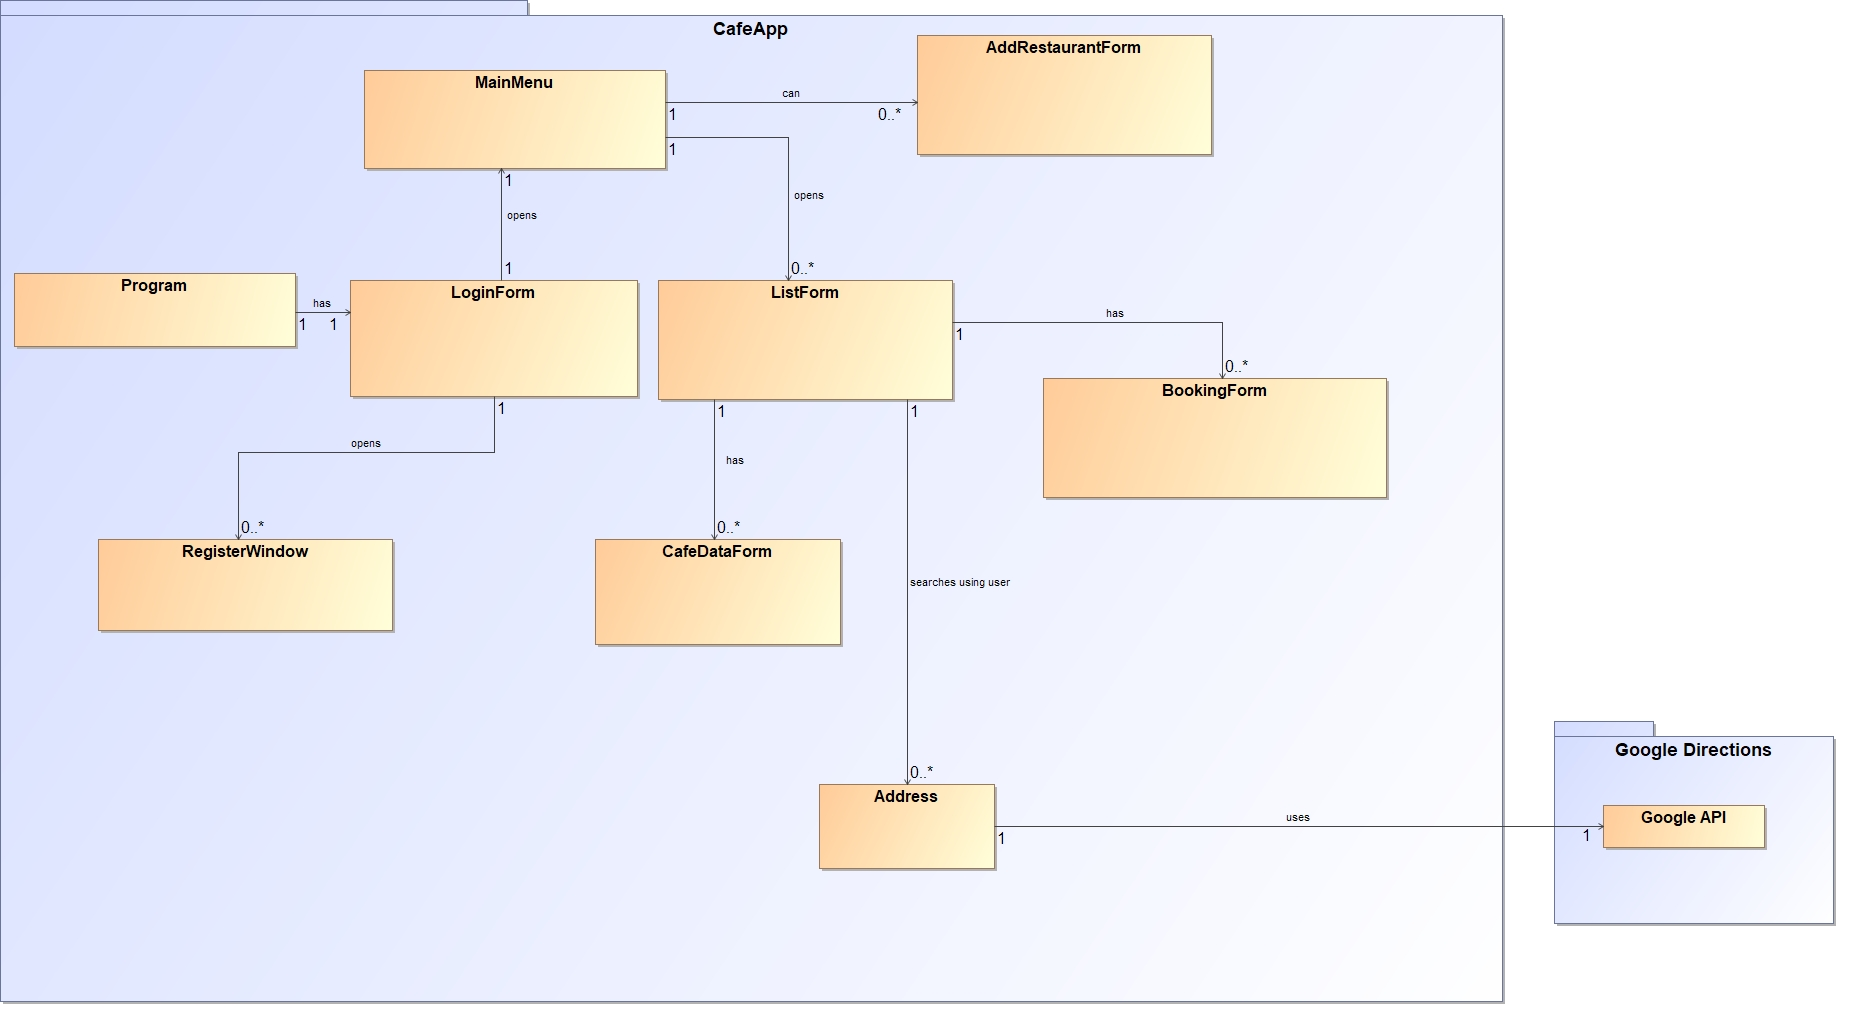
\includegraphics[width=\textwidth,height=\textheight,keepaspectratio]{img/Model} 
    \caption{Klasių diagrama}
    \label{img:Model}
\end{figure}
%OBJEKTU DIAGRAMA
\subsubsection{Objektų diagrama}

\section{Medžiagos darbo tema dėstymo skyriai}
Medžiagos darbo tema dėstymo skyriuose pateikiamos nagrinėjamos temos detalės:
pradinė medžiaga, jos analizės ir apdorojimo metodai, sprendimų įgyvendinimas,
gautų rezultatų apibendrinimas. Šios dalies turinys labai priklauso nuo darbo
temos. Skyriai gali turėti poskyrius ir smulkesnes sudėtines dalis, kaip
punktus ir papunkčius.

Medžiaga turi būti dėstoma aiškiai, pateikiant argumentus. Tekstas dėstomas
trečiuoju asmeniu, t.y. rašoma ne „aš manau“, bet „autorius mano“, „autoriaus
nuomone“. Reikėtų vengti informacijos nesuteikiančių frazių, pvz., „...kaip jau
buvo minėta...“, „...kaip visiems žinoma...“ ir pan., vengti grožinės literatūros
ar publicistinio stiliaus, gausių metaforų ar panašių meninės išraiškos
priemonių.

\subsection{Poskyris}
Citavimo pavyzdžiai: cituojamas vienas šaltinis \cite{PvzStraipsnLt}; cituojami
keli šaltiniai \cite{PvzStraipsnEn, PvzKonfLt, PvzKonfEn, PvzKnygLt, PvzKnygEn,
PvzElPubLt, PvzElPubEn, PvzMagistrLt, PvzPhdEn}.

\begin{enumerate}
	\item Pirmas elementas
	\item Antras elementas
\end{enumerate}

Lorem ipsum dolor sit amet, consectetur adipiscing elit. Curabitur at mauris sit amet nisi vestibulum tincidunt non vel mi. Pellentesque lacinia, sapien id sollicitudin egestas, diam erat dapibus justo, a cursus arcu nunc feugiat sapien. Mauris elit lorem, egestas at nisl at, consequat tempus nisi. Aliquam congue consectetur lorem ut venenatis. Suspendisse scelerisque eros ac sapien pulvinar, id fermentum sem bibendum. Phasellus rhoncus nec tellus quis gravida. Fusce at nibh porta, sodales ipsum quis, facilisis velit. Phasellus semper laoreet magna, eget eleifend massa. Donec sollicitudin risus risus, sodales dignissim ex bibendum et. Aliquam neque lectus, posuere vitae suscipit et, hendrerit eu mauris. Integer cursus neque ex, sed molestie ex suscipit et. Phasellus eget quam id arcu tincidunt fringilla eget eu tortor. In hac habitasse platea dictumst.



\subsubsection{Skirsnis}
\subsubsubsection{Straipsnis}
\subsubsection{Skirsnis}
\section{Skyrius}
\subsection{Poskyris}
\subsection{Poskyris}

\sectionnonum{Rezultatai ir išvados}
Rezultatų ir išvadų dalyje turi būti aiškiai išdėstomi pagrindiniai darbo
rezultatai (kažkas išanalizuota, kažkas sukurta, kažkas įdiegta) ir pateikiamos
išvados (daromi nagrinėtų problemų sprendimo metodų palyginimai, teikiamos
rekomendacijos, akcentuojamos naujovės).


%% PAKEISTAS PAVADINIMAS Į 'Šaltiniai'
\printbibliography[heading=bibintoc, title=Šaltiniai]  % Šaltinių sąraše nurodoma panaudota
% literatūra, kitokie šaltiniai. Abėcėlės tvarka išdėstomi darbe panaudotų
% (cituotų, perfrazuotų ar bent paminėtų) mokslo leidinių, kitokių publikacijų
% bibliografiniai aprašai.  Šaltinių sąrašas spausdinamas iš naujo puslapio.
% Aprašai pateikiami netransliteruoti. Šaltinių sąraše negali būti tokių
% šaltinių, kurie nebuvo paminėti tekste.

% \sectionnonum{Sąvokų apibrėžimai}
\sectionnonum{Santrumpos}
Sąvokų apibrėžimai ir santrumpų sąrašas sudaromas tada, kai darbo tekste
vartojami specialūs paaiškinimo reikalaujantys terminai ir rečiau sutinkamos
santrumpos.

\appendix  % Priedai
% Prieduose gali būti pateikiama pagalbinė, ypač darbo autoriaus savarankiškai
% parengta, medžiaga. Savarankiški priedai gali būti pateikiami ir
% kompaktiniame diske. Priedai taip pat numeruojami ir vadinami. Darbo tekstas
% su priedais susiejamas nuorodomis.

\section{Neuroninio tinklo struktūra}
\begin{figure}[H]
    \centering
    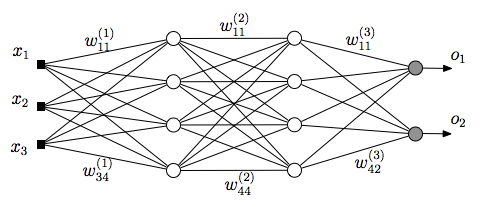
\includegraphics[scale=0.5]{img/MLP}
    \caption{Paveikslėlio pavyzdys}
    \label{img:mlp}
\end{figure}


\section{Eksperimentinio palyginimo rezultatai}
% tablesgenerator.com - converts calculators (e.g. excel) tables to LaTeX
\begin{table}[H]\footnotesize
  \centering
  \caption{Lentelės pavyzdys}
  {\begin{tabular}{|l|c|c|} \hline
    Algoritmas & $\bar{x}$ & $\sigma^{2}$ \\
    \hline
    Algoritmas A  & 1.6335    & 0.5584       \\
    Algoritmas B  & 1.7395    & 0.5647       \\
    \hline
  \end{tabular}}
  \label{tab:table example}
\end{table}

\end{document}
